% =====================================================================
%  EpiForecast-MX  --  MICAI 2026 Proceedings Submission
%  Springer LNCS / LNAI format  (llncs.cls v2.24, official 2024 release)
%
%  This master file is the CAMERA-READY version (with authors).
%  Blocks that differ for the DOUBLE-BLIND REVIEW version are marked
%  with  "% >>> REVIEW:"  /  "% >>> CAMERA-READY:"  comments. To produce
%  the anonymous review PDF, comment out the CAMERA-READY block and
%  uncomment the REVIEW block at each marked location (author block,
%  code-availability sentence, acknowledgments, disclosure, named
%  institutions in the ethics statement).
%
%  OVERLEAF SETUP
%  --------------
%  1. Upload llncs.cls, splncs04.bst and the Figures/ folder alongside
%     this .tex.  2. Compiler = pdfLaTeX.  3. Run pdfLaTeX three times
%     (or auto-recompile) so all \ref{} cross-references resolve.
%
%  PAGE GEOMETRY: the LNCS book trim is fixed by llncs.cls. Do NOT load
%  the geometry package or override the margins -- Springer typesetters
%  reject any layout that deviates from llncs.cls defaults.
% =====================================================================
\documentclass[runningheads]{llncs}

% Set the PDF media box to A4 (Springer LNCS final format). Applied via
% \AtBeginDocument so it overrides the size llncs fixes at \begin{document}.
% Only the physical page size changes; the fixed llncs text block stays
% anchored at the top-left origin, so margins and geometry are untouched.
\AtBeginDocument{\pdfpagewidth=210mm \pdfpageheight=297mm}

% Capa de texto: sin esto el PDF no describe las ligaduras (fi, ff, fl) y el texto se
% extrae roto -- "cutoff" se copia como "cuto". Lo resuelve `cmap` mas abajo (fuentes CM
% en T1); estas dos lineas cubren ademas los glifos con nombre estandar. No cambian ni un
% pixel de la composicion: solo arreglan buscar y copiar en el PDF de las actas.
\input{glyphtounicode}
\pdfgentounicode=1

% cmap va ANTES de fontenc: genera los CMap ToUnicode de las fuentes CM en T1, que es
% lo que de verdad arregla la extraccion de ligaduras aqui (glyphtounicode solo cubre
% nombres de glifo estandar). Sin esto "cutoff" se copia como "cuto".
\usepackage{cmap}
\usepackage[T1]{fontenc}
\usepackage[utf8]{inputenc}
\usepackage[english]{babel}
\usepackage{graphicx}
\usepackage{booktabs}
\usepackage{amsmath}
\usepackage{amssymb}
\usepackage{array}
\usepackage{tikz}
\usetikzlibrary{positioning,arrows.meta,shapes.geometric,fit,backgrounds,calc}
\usepackage{xcolor}
% Corresponding-author marker: Springer recommends \usepackage{bbding}\Envelope.
% Fallback keeps the file compilable where bbding is unavailable (e.g. minimal
% TeX installs); on Overleaf the bbding glyph is used.
\IfFileExists{bbding.sty}{\usepackage{bbding}}{\providecommand{\Envelope}{$\boxtimes$}}
\usepackage{hyperref}
\renewcommand\UrlFont{\color{black}\rmfamily}
\urlstyle{rm}

\graphicspath{{Figures/}}

\newcommand{\smape}{sMAPE}
\newcommand{\mase}{MASE}
\newcommand{\rmse}{RMSE}
\newcommand{\mae}{MAE}

\begin{document}

% =====================================================================
\title{Forecasting Weekly Depression Incidence in Mexico:
       A Multi-Model Framework with Auditable
       Per-Series Model Selection}

\titlerunning{Forecasting Depression in Mexico}

% >>> CAMERA-READY author block (active). For REVIEW, comment this out
%     and uncomment the anonymous block below.
% ORCID de los cinco, verificados con sus titulares (20-ago-2026).
% \orcidID lo define llncs.cls; la clase ya los suprime del indice y del titulillo.
% Nombres, orden, afiliaciones y correos contrastados con la ficha de CMT (consultada
% 20-ago-2026): la carta de aceptacion exige que el camera-ready y CMT coincidan.
% La forma de Ruth y su afiliacion reproducen su instruccion expresa del 20-ago-2026;
% CMT conserva una forma abreviada anterior y debe actualizarse antes de la entrega.
\author{Javier Rebull-Saucedo\inst{1}\orcidID{0009-0008-2089-5274}(\Envelope) \and
        Juan P\'erez-Nava\inst{1}\orcidID{0009-0005-6708-5541} \and
        Luis S\'anchez-Salazar\inst{1}\orcidID{0009-0009-6101-8072} \and
        Grettel Barcel\'o-Alonso\inst{1}\orcidID{0009-0004-3373-6441} \and
        Ruth P\'erez-Hern\'andez\inst{2}\orcidID{0000-0003-3261-1220}}
\authorrunning{J. Rebull-Saucedo et al.}
% Afiliacion segun TEC-II-05 "Lineamientos para la afiliacion institucional" (v.03,
% vigente 2025): el nombre es "Tecnologico de Monterrey", en espanol y SIN ACENTO --
% la excepcion existe para que los sistemas de indexacion no lo corrompan--, sin siglas,
% sin abreviaturas y sin traducciones. El campus NO se agrega (seccion III); el programa
% MNA se menciona en Acknowledgments, que es donde el lineamiento lo permite (seccion V).
% "ITESM" figura entre las afiliaciones NO aceptadas (seccion VI).
\institute{Tecnologico de Monterrey, Monterrey, Mexico\\
           \email{rebull@outlook.com}, \email{jcpn@me.com},\\
           \email{luisgss10@hotmail.com}, \email{gbarcelo@tec.mx}
           \and
           % Organo declarado por la propia autora (20-ago-2026); no se traduce. El cargo
           % ("Investigadora Asociada") no va aqui: el bloque de LNCS marca instituciones,
           % no puestos, y el superindice debe apuntar a la institucion.
           Instituto Mexicano del Seguro Social, \'Organo de Operaci\'on Administrativa\\
           Desconcentrada Estatal Guerrero, Mexico\\
           \email{ruth.perezher@imss.gob.mx}}
% >>> REVIEW (double-blind) author block (inactive):
% \author{Anonymous Author(s)}
% \authorrunning{Anonymous}
% \institute{Affiliations withheld for double-blind review}

\maketitle

% =====================================================================
\begin{abstract}
Weekly forecasting of psychiatric demand is hard because surveillance
signals are heterogeneous across regions, sex strata, and time, so no single
forecasting paradigm performs uniformly well. Rather than imposing one
algorithm across an entire surveillance system, we present a
deterministic, auditable framework that selects, for each series, the
model best supported by its own evidence. The framework draws on a
library of forecasters with deliberately different inductive
assumptions---a structural additive decomposition, a probabilistic
recurrent network, and two tree-based hybrids---so that the candidate pool
spans diverse temporal representations. A transparent rule then selects
one model per series based on cross-validated accuracy, can reassign
low-incidence series to a regional model, and records every decision in a
justified selection log. We instantiate it for weekly depression
incidence (CIE-10 F32) across Mexico's 32 federal entities, using public
bulletins of the National Epidemiological Surveillance System (SINAVE),
and validate it twice: by rolling-origin cross-validation over a decade of
weekly observations and a prospective out-of-sample assessment against the
2026 bulletins released after the training cutoff. A leave-one-model-out
ablation shows that the candidate pool is not what carries the result, and
that the cross-validated ranking does not transport to the prospective
window. The contribution is therefore not that several models beat one,
but that an auditable mechanism detects when a frozen assignment stops
transporting and revises it using only prior observations. The framework
is reproducible and extends to conditions with heterogeneous behavior.

\keywords{Depression \and Time series forecasting \and
          Probabilistic recurrent networks \and Multi-model
          forecasting \and Epidemiological surveillance \and
          Model selection.}
\end{abstract}

% =====================================================================
\section{Introduction}
\label{sec:intro}
% =====================================================================

Depression is a leading cause of disability worldwide and imposes a major
burden on public health systems~\cite{santomauro2021}.
In Mexico, it affects an estimated 8--10 million people, and the
National Epidemiological Surveillance System (SINAVE) records over
150{,}000 new cases of depressive episode (CIE-10 F32) per
year~\cite{sinave2026}. Despite the routine availability of weekly
case counts, psychiatric-service planning remains largely
\emph{reactive}: capacity is adjusted only after demand surges are
already visible in the bulletin, producing recurrent saturation
windows during the February--May period.

Accurate weekly federal-entity forecasts would make this planning
\emph{proactive}: a reliable 52-week-ahead trajectory would allow
authorities to pre-position staff before seasonal peaks, size programs
by state, and time help-seeking campaigns for quieter months. The
problem is challenging precisely where forecasts are most
consequential. The depression signal is highly
heterogeneous: case loads differ by orders of magnitude across
entities, are sharply skewed by sex, and range from smooth
metropolitan series to volatile low-volume states in a panel marked
by a COVID-19 regime change and a post-pandemic level shift. No single
paradigm accommodates all of these at once: structural decompositions
excel on smooth aggregates but lag on noisy series, whereas
representation-learning models share structure across series but can
overreact on smooth aggregates. Deployment also raises a trust
problem: a model chosen on historical cross-validation can quietly lose
its edge once the live signal shifts, so an institution needs a
selection it can audit and revise, not a one-off leaderboard winner.

We address this problem with a \textbf{multi-model forecasting framework},
referred to throughout as \emph{the proposed framework}. Rather than
committing to one model
family, it trains four forecasters with complementary inductive
assumptions for each series and selects one model per series through a
deterministic, auditable rule, so that the paradigm best supported by
a given series produces that series' forecast. Although evaluated
here on depression, the framework is designed for epidemiological
surveillance in general: choosing one model per series is a direct
response to the heterogeneity that makes any single architecture
unlikely to dominate across the many conditions a surveillance system
monitors.

The main contributions of this study are threefold: (i)~we present
and empirically evaluate a multi-model forecasting framework for
psychiatric surveillance that places structural, recurrent, and
tree-based forecasters behind a single interface, enabling a
head-to-head, per-series comparison under one rolling-origin protocol; (ii)~we
introduce a deterministic, auditable per-series model-selection
strategy that ranks candidates on cross-validated symmetric error with
scale-free and large-error tie-breakers and a transparent low-incidence
regional fallback, producing a fully justified, revisable selection
log---an auditable selection mechanism built for trustworthy deployment
under distribution shift rather than a one-off leaderboard choice; and (iii)~we provide a nationwide empirical
characterization, over 111 series--stratum combinations and 626 weeks of
SINAVE data, of the regional, demographic, and temporal
heterogeneity of the depression signal and of the conditions under which
each forecasting paradigm prevails. A central finding is that the cross-validated ranking is a
\emph{selection} signal, not an out-of-sample guarantee: per-series
accuracy degrades on live 2026 data, a degradation the revisable
rule absorbs by reassigning models as the signal accumulates,
substantiated by the first eighteen epidemiological weeks of 2026.

% =====================================================================
\section{Foundations and Related Work}
\label{sec:related}
% =====================================================================

\subsection{Epidemiological Time-Series Forecasting}

Incidence forecasting has progressed from linear, series-by-series
statistical models to global, representation-learning architectures
that share parameters across many related series. The Box--Jenkins
autoregressive integrated moving average (ARIMA) family~\cite{box2015}
remains a
standard baseline, but its linearity and stationarity assumptions
limit performance on non-stationary public-health signals subject to
regime changes. Exponential-smoothing state-space models
(ETS)~\cite{hyndman2008} offer flexible additive or multiplicative
decompositions but treat each series independently.
Prophet~\cite{taylor2018} popularized an additive decomposition with
explicit trend, seasonality, and holiday components and is robust to
missing data and outliers, making it a frequent default in
public-health pipelines; however, its smooth additive structure can
underfit the volatile low-count series typical of small federal
entities. Recurrent neural networks (RNNs), particularly long
short-term memory (LSTM) networks, have shown clear
advantages for epidemiological series: Chimmula and
Zhang~\cite{chimmula2020} applied LSTMs to COVID-19 incidence in
Canada, outperforming classical baselines over short horizons,
although such data-hungry models can overreact on smooth, high-volume
aggregates for which simpler decompositions may already suffice. For
public-health surveillance specifically, collaborative forecasting
efforts have shown that systematic, reproducible evaluation of
probabilistic forecasts is feasible at a national
scale~\cite{reich2019,cramer2022}. More recent architectures push long-horizon
accuracy further---for example, the hierarchical-interpolation network
N-HiTS~\cite{challu2023nhits}---and large pretrained \emph{foundation}
models for time series, such as Chronos~\cite{ansari2024chronos},
forecast across many domains with little or no task-specific training;
their behavior on the sparse, regime-shifting panels typical of
epidemiological surveillance remains largely untested.

\subsection{Foundations of Multi-Model Forecasting}

The case for combining heterogeneous forecasters is well established.
Salinas et~al.~\cite{salinas2020} introduced DeepAR, a global
probabilistic autoregressive RNN that \emph{learns} across a panel of
related series and emits a full predictive
distribution at each step; recent surveys of deep learning for
forecasting situate such global models within a broad design
space~\cite{benidis2022,lim2021,hewamalage2021}. Large-scale
empirical evidence from the M4 and M5 forecasting competitions---open
benchmarks spanning 100{,}000 cross-domain series and a
large hierarchical retail-sales corpus, respectively---shows that
machine-learning and hybrid methods are competitive with, and often
outperform, classical univariate methods across heterogeneous
collections, and that combinations are particularly
robust~\cite{makridakis2020,makridakis2022}, including automated
ensembles tuned to weekly series~\cite{godahewa2023}. Combining the explicit
components of additive decompositions with the nonlinear capacity of
gradient-boosted decision trees (GBDTs) has proven effective in retail
and energy forecasting~\cite{hyndman2018forecasting}, and Prophet--neural
hybrids have improved pandemic incidence forecasts~\cite{dash2024}. Stacked
generalization~\cite{wolpert1992} formalizes the learning of a meta-model
over heterogeneous base learners. These foundations motivate a
design in which structural, statistical, and learning-based
assumptions coexist and a principled rule decides between them per
series.

\paragraph{Why these four candidates.}
The pool samples the design space above rather than enumerating it: one
representative per family of inductive assumption, chosen so that the
selection rule adjudicates between genuinely different beliefs about the
signal rather than between variants of one. Prophet contributes an
explicit structural decomposition of trend and annual seasonality;
DeepAR contributes a global probabilistic model that pools strength
across the panel and emits a predictive distribution; and the two
tree-based hybrids contribute nonlinear responses to calendar and lag
features that neither of the first two represents, one blended with a
structural component and one stacked over heterogeneous experts. Two
further candidates were implemented and evaluated under the identical
protocol and then left out of the deployed pool: a tuned Auto-ARIMA with
Fourier annual terms, as the classical baseline the family above
motivates, and PatchTST, as a patching transformer representative of the
recent long-horizon architectures. Both are reported in
Table~\ref{tab:aggmetrics} rather than hidden: neither reached the
accuracy of the retained candidates on this panel, and PatchTST in
particular did not repay its tuning cost at the 111-series scale.
Foundation models such as Chronos~\cite{ansari2024chronos} were not
evaluated here and remain open. The pool is therefore a documented
sample of the space, not a claim of completeness---and
Sect.~\ref{ssec:ablation} tests how much of the result actually depends
on it.

\subsection{Depression and Mental-Health Surveillance}

The burden of depression in Mexico has been quantified through the
Global Burden of Disease study~\cite{garciapacheco2024}, and the
COVID-19 pandemic produced a measurable global increase in
depressive-disorder burden~\cite{santomauro2021}. Sex-related
disparities in reported incidence are well established
clinically~\cite{albert2015}. To our knowledge, no prior work has
applied a multi-model forecasting framework with auditable per-series
model selection to the SINAVE depression panel at federal-entity
granularity while also providing a prospective out-of-sample
evaluation.

% =====================================================================
\section{Materials and Methods}
\label{sec:method}
% =====================================================================

\subsection{Data Characterization}
\label{ssec:data}

The study uses weekly case counts of \emph{depressive episode}, the
category the WHO International Classification of Diseases, 10th revision
(ICD-10) codes as \textbf{F32}: a first, single episode of depressed
mood with loss of interest and reduced energy, graded mild, moderate, or
severe, and distinct from recurrent depressive disorder (F33). SINAVE
labels it with the Spanish acronym of the same classification, CIE-10.
Counts are as reported in the SINAVE bulletin
by the Direcci\'on General de
Epidemiolog\'ia~\cite{sinave2026}, Mexico's consolidated public health
surveillance system. After calendar alignment under the
SINAVE epidemiological-week convention,\footnote{The SINAVE calendar
is similar but not identical to the ISO~8601 and CDC Morbidity and
Mortality Weekly Report (MMWR) week
conventions. We use the calendar as published in the bulletin and do
not re-index against either external standard.} the harmonized panel
contains \textbf{626 weekly observations per series}, spanning
2014-W02 through 2025-W53. Epidemiological
week~1 of 2014 was unavailable in the retrieved archive, so 2014
contributes 52 weeks; 2020 and 2025 each contain 53 epidemiological
weeks, giving $626 = 10{\times}52 + 2{\times}53$. Records are
disaggregated by sex (women and men) and aggregated into an overall
total (general). We analyze the 32 federal entities,
four socio-urban regions defined by population density and INEGI
demographic indicators (\emph{Metropolitana alta}, \emph{Urbana
media}, \emph{Sur-Sureste vulnerable}, \emph{Rural / dispersa}), and a
national series, yielding $37 \times 3 = 111$ series--stratum
combinations.

\paragraph{Temporal and seasonal structure.}
Figure~\ref{fig:temporal} shows the national series. Three regimes are
visible: a stable 2014--2018 baseline; the COVID-19 disruption of
2020--2021, when both reporting capacity and clinical demand shifted
abruptly; and a post-pandemic regime in 2022--2025 that exceeds
pre-pandemic levels. The series exhibits clear intra-annual
seasonality, with recurring annual peaks between epidemiological
weeks 8 and 20 (February--May).

\begin{figure}[t]
\centering
% ALT-TEXT (accessibility / proofing): Two-panel chart: (a) annual reported depression (CIE-10 F32) cases 2014-2026 as bars; (b) weekly national series with the COVID-19 disruption window shaded.
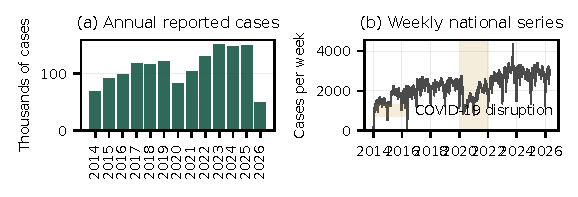
\includegraphics[width=0.80\textwidth]{fig01_temporal_distribution.pdf}
\caption{Depression (CIE-10 F32) temporal distribution. (a) Annual
reported cases 2014--2026 (2026 is year-to-date). (b) Weekly national
series; the COVID-19 disruption window is highlighted in gold. The
post-2022 level shift and the recurring February--May peaks motivate
models that adapt across regimes.}
\label{fig:temporal}
\end{figure}

\paragraph{Spatial, regional, and demographic heterogeneity.}
State-level case loads vary by more than two orders of magnitude:
the highest-volume entities (Ciudad de
M\'exico, Jalisco, Estado de M\'exico, Chihuahua, and Veracruz)
together account for
about 40\% of the cumulative caseload,
while sparsely populated southern states are lower but more volatile,
which penalizes single-series baselines. Women account for 74.0\% of
reported cases against 26.0\% in men over 2014--2025, exceeding the
1.5--2$\times$ female prevalence of major depressive
disorder~\cite{albert2015}; because the data are \emph{reported incidence},
this likely reflects both clinical patterns and male underreporting.
We forecast the three strata separately and revisit the gap in
Sect.~\ref{sec:discussion}. Based on the indicators available for
measurement---a median annual coefficient of
variation below 0.25, negligible missing weeks, and a well-contained
COVID-19 window---this panel is unusually clean and therefore amenable to
data-driven sequence models.

\subsection{Proposed Framework}
\label{ssec:framework}

\paragraph{Rationale.}
The heterogeneity documented above motivates a design that does not
commit to one inductive bias. For each series, we train four
forecasters whose assumptions are deliberately complementary, and a
deterministic rule selects among them. The methodological core
is not any individual forecaster---all four are established models---but
the principled, per-series choice among them: each series is matched to
the inductive bias its own history supports through a deterministic and
fully auditable rule, rather than through a global or hand-tuned
commitment. A structural additive model captures explicit trend and
seasonality and performs well on smooth aggregates; a probabilistic
recurrent network with a flexible autoregressive structure performs
well on many noisy state series; and two tree-based hybrids add
nonlinear interactions among calendar, lag, and demographic features. The four forecasters are
exposed through a single, common interface, so that the selection rule
operates uniformly across all of them (Fig.~\ref{fig:pipeline}).

\begin{itemize}
\item \textbf{Probabilistic recurrent network (DeepAR)}~\cite{salinas2020,alexandrov2020}:
an autoregressive recurrent network that emits a Student-$t$
distribution whose mean is the point forecast. Each federal-entity and
regional series is fit with its own DeepAR model; the national
aggregate uses a single DeepAR trained jointly over the 32 state series,
with the per-state forecasts summed to give the national total. A controlled
comparison (Sect.~\ref{ssec:eval}) shows that joint training adds only a
small margin over per-series fitting, so the per-series variant is used
at the federal-entity level.
\item \textbf{Structural additive model (Prophet)}~\cite{taylor2018}:
piecewise-linear trend with automatic change points plus Fourier annual
seasonality, fit to the $\log(1{+}y)$ rate per 100{,}000 inhabitants
to stabilize variance across population sizes.
\item \textbf{Parallel hybrid (Ensemble)}: an XGBoost
regressor~\cite{chen2016} using calendar features as well as lagged
and rolling-window statistics (lags $\{1,2,4,8,13,26,52\}$ weeks,
spanning short-term momentum, quarterly structure, and the annual
cycle), blended with Prophet in count space as
$\hat{y}_t=\alpha\hat{y}^{P}_t+(1{-}\alpha)\hat{y}^{XGB}_t$ with
$\alpha$ fit on out-of-fold predictions, so that Prophet's smooth
trend and seasonality complement XGBoost's nonlinear lag interactions.
\item \textbf{Stacked hybrid (Stacking)}: Prophet, ETS and
LightGBM~\cite{ke2017} experts---two structural/statistical views of
trend and seasonality plus one nonlinear learner---combined by a
nonnegative ElasticNet meta-learner over out-of-fold predictions; the
nonnegativity constraint keeps the learned weights interpretable as
positive contributions and stable on short series.
\end{itemize}

\paragraph{Low-incidence regional fallback.}
Series with structurally low historical incidence---cumulative count
below 5 cases in the 52 weeks immediately preceding the forecast
origin---are reassigned to the model selected for their socio-urban
region (Fig.~\ref{fig:pipeline}). For such near-zero series, percentage
metrics are dominated by noise, so a regional model
estimated from a denser signal is a safer default. The rule depends
only on past observations and is therefore free of look-ahead bias. In
the depression panel studied here, no series falls below the threshold,
so the fallback is not activated; it is retained as a safeguard for
sparser conditions in the SINAVE catalog.

\begin{figure}[t]
\centering
% ALT-TEXT (accessibility / proofing): Flow diagram of the proposed framework: SINAVE bulletin -> cleaning and feature engineering -> rolling-origin cross-validation -> four candidate models trained in parallel per series (DeepAR, Prophet, Ensemble, Stacking) -> deterministic selector (sMAPE -> MASE -> RMSE) -> low-incidence gate routing either to a regional model or to the locked 52-week forecast.
% IMSS palette
\definecolor{ImssGreen}{HTML}{0A4F3C}
\definecolor{ImssGold}{HTML}{B8860B}
\definecolor{ImssWine}{HTML}{880E4F}
\definecolor{ImssIndigo}{HTML}{1A237E}
\definecolor{ImssOrange}{HTML}{C75300}
\definecolor{ImssNavy}{HTML}{0D2A4F}
\definecolor{ImssGray}{HTML}{4A4A4A}
\resizebox{\textwidth}{!}{%
\begin{tikzpicture}[
    >={Stealth[length=2.6mm, width=1.8mm]},
    every node/.style={font=\small},
    data/.style={rectangle, rounded corners=4pt,
        draw=ImssGreen, line width=0.9pt, fill=ImssGreen, text=white,
        minimum width=22mm, minimum height=12mm, align=center,
        font=\small\bfseries},
    output/.style={rectangle, rounded corners=4pt,
        draw=ImssNavy, line width=0.9pt, fill=ImssNavy, text=white,
        minimum width=22mm, minimum height=12mm, align=center,
        font=\small\bfseries},
    cand/.style={rectangle, rounded corners=4pt,
        draw=ImssGray, line width=1pt, fill=ImssGray!6,
        text=ImssGray!20!black,
        minimum width=21mm, minimum height=10mm, align=center,
        font=\small\bfseries},
    selector/.style={rectangle, rounded corners=4pt,
        draw=ImssGold, line width=1.4pt, fill=ImssGold!12,
        text=ImssGold!35!black,
        minimum width=27mm, minimum height=14mm, align=center,
        font=\small\bfseries},
    gate/.style={diamond, aspect=2.1, draw=ImssWine, line width=1pt,
        fill=ImssWine!8, text=ImssWine!55!black,
        inner sep=1pt, align=center, font=\scriptsize\bfseries},
    regio/.style={rectangle, rounded corners=4pt,
        draw=ImssWine, line width=1pt, fill=ImssWine!8,
        text=ImssWine!55!black, minimum width=22mm, minimum height=10mm,
        align=center, font=\scriptsize\bfseries},
    flow/.style={->, line width=0.9pt, draw=ImssGray!55, rounded corners=2pt},
    flowmain/.style={->, line width=1.5pt, draw=ImssGreen!80!black,
        rounded corners=2pt},
    stage/.style={font=\footnotesize\itshape, text=ImssGray}
]
\node[data] (sinave) {SINAVE\\bulletin\\[0.4mm]\scriptsize\mdseries 2014--2025};
\node[data, right=10mm of sinave] (clean) {Clean +\\features};
\node[data, right=10mm of clean]  (cv)    {Rolling-\\origin CV};

\node[cand, right=20mm of cv, yshift=18mm]  (deepar)  {DeepAR\\[0.2mm]\scriptsize\mdseries global RNN};
\node[cand, right=20mm of cv, yshift=6mm]   (prophet) {Prophet\\[0.2mm]\scriptsize\mdseries additive};
\node[cand, right=20mm of cv, yshift=-6mm]  (ens)     {Ensemble\\[0.2mm]\scriptsize\mdseries $+$XGBoost};
\node[cand, right=20mm of cv, yshift=-18mm] (stack)   {Stacking\\[0.2mm]\scriptsize\mdseries 3 experts};

\node[selector, right=22mm of prophet, yshift=-6mm] (sel)
     {Model\\selection\\[0.4mm]\scriptsize\mdseries
      \smape\ $\to$ \mase\ $\to$ \rmse};

\node[gate, right=14mm of sel] (gate) {Low-\\incidence?};
\node[regio, below=8mm of gate] (regio) {Regional\\model};
\node[output, right=14mm of gate] (out)
     {Locked\\forecast\\[0.4mm]\scriptsize\mdseries 52 weeks};

\begin{pgfonlayer}{background}
\node[fit=(deepar)(prophet)(ens)(stack),
      inner xsep=4mm, inner ysep=3mm, rounded corners=6pt,
      fill=ImssGray!4, draw=ImssGray!25, line width=0.4pt, dashed] (engbox) {};
\end{pgfonlayer}
\node[stage, anchor=south] at (engbox.north) [yshift=0.4mm]
     {Four candidate models, trained in parallel per series};

\draw[flowmain] (sinave) -- (clean);
\draw[flowmain] (clean)  -- (cv);
\draw[flow] (cv.east) to[out=18,  in=180] (deepar.west);
\draw[flow] (cv.east) to[out=6,   in=180] (prophet.west);
\draw[flow] (cv.east) to[out=-6,  in=180] (ens.west);
\draw[flow] (cv.east) to[out=-18, in=180] (stack.west);
\draw[flow] (deepar.east)  to[out=0, in=165] (sel.west);
\draw[flow] (prophet.east) to[out=0, in=178] (sel.west);
\draw[flow] (ens.east)     to[out=0, in=190] (sel.west);
\draw[flow] (stack.east)   to[out=0, in=205] (sel.west);
\draw[flowmain] (sel) -- (gate);
\draw[flowmain] (gate) -- node[above, font=\scriptsize, text=ImssGreen!50!black]{no} (out);
\draw[flow] (gate) -- node[right, font=\scriptsize, text=ImssWine!55!black]{yes} (regio);
\draw[flow] (regio.east) to[out=0, in=250] (out.south);
\end{tikzpicture}%
}
\caption{Proposed framework. Four candidate models with complementary
inductive assumptions are trained in parallel per series; a
deterministic rule selects one on cross-validated \smape\ (with
\mase\ and \rmse\ tie-breakers), after which structurally low-incidence
series are routed to their regional model before the 52-week forecast
is locked.}
\label{fig:pipeline}
\end{figure}

\subsection{Evaluation Protocol}
\label{ssec:eval}

\paragraph{Cross-validation.}
Every series--stratum combination is evaluated by rolling-origin
cross-validation with five folds, a 52-week horizon, and a 13-week
(one-quarter) stride; the training window expands at each fold.
Metrics are accumulated across folds and weeks, and we report the
median across folds per \{series, stratum, model\} triple.

\paragraph{Metrics and their rationale.}
Let $y_t$ be the observed value and $\hat{y}_t$ the point forecast at
step $t$ over a horizon $H$. We use four complementary metrics---root
mean squared error (\rmse), mean absolute error (\mae), symmetric
mean absolute percentage error (\smape), and mean absolute scaled
error (\mase)---defined in Eqs.~(\ref{eq:rmse_mae})--(\ref{eq:smape_mase}),
so that no single artifact dominates the selection.
\begin{equation}
\rmse = \sqrt{\tfrac{1}{H}\textstyle\sum_{t=1}^{H}(y_t-\hat{y}_t)^{2}},
\qquad
\mae = \tfrac{1}{H}\textstyle\sum_{t=1}^{H}|y_t-\hat{y}_t|,
\label{eq:rmse_mae}
\end{equation}
\begin{equation}
\smape = \frac{100}{H}\sum_{t=1}^{H}
\frac{|y_t-\hat{y}_t|}{(|y_t|+|\hat{y}_t|)/2},
\qquad
\mase = \frac{\frac{1}{H}\sum_{t=1}^{H}|y_t-\hat{y}_t|}
            {\frac{1}{n-52}\sum_{t=53}^{n}|y_t-y_{t-52}|}.
\label{eq:smape_mase}
\end{equation}
\smape\ is scale-normalized and symmetric, making it comparable across
entities with very different volumes, and it is our primary criterion;
\mase~\cite{hyndman2006} normalizes by a 52-week seasonal-naive
benchmark, so a value below~1 beats seasonal persistence regardless of
scale; \rmse\ penalizes large errors, and \mae\ is an interpretable
case-count error. Excluding the W53 weeks from the two 53-week years
shifts every median \mase\ by less than $0.005$ and leaves the ranking
unchanged.

\paragraph{Leakage prevention.}
Temporal leakage is controlled throughout: the rolling-origin splits
are strictly expanding; lag and rolling features never reference an
observation later than the forecast origin (multi-step rollout fills
$h{>}1$ lags \emph{recursively} with predictions, never future values);
demographic covariates are pre-origin annual estimates; and the
low-incidence fallback depends only on past counts. The 2026 bulletins
of Sect.~\ref{sec:validation} were used \emph{exclusively} for
evaluation: no 2026 observation was used to train, tune, or reselect
any model, and all hyperparameters, architectures, and the selection rule were
fixed on data through 2025-W53. We therefore describe the evaluation as
\emph{out-of-sample} rather than \emph{blind}; the guarantee is the
temporal separation described above. As a leakage check, an otherwise
identical global-versus-local (single-series) DeepAR pair on eight
states improved the
median \smape\ by only ${\sim}5\%$ ($24.9$ vs.\ $26.3$): a modest,
legitimate cross-learning gain, not an information
leak.\footnote{This controlled pair uses a lightweight identical
configuration to isolate the global-versus-local effect; its absolute
errors exceed those of the production-configured model in
Table~\ref{tab:aggmetrics}.}

\paragraph{Baselines.}
Beyond the four candidate models of Sect.~\ref{ssec:framework}, the
52-week seasonal-naive benchmark is the denominator of \mase\ and is
reported explicitly (Table~\ref{tab:aggmetrics}), together with two
baselines reimplemented under the identical CV: a tuned Auto-ARIMA
with Fourier annual terms and a PatchTST transformer.

\paragraph{Model selection strategy.}
For a series--stratum combination, let $\mathcal{E}$ be the candidate
set and, for each model $e\in\mathcal{E}$, let $s_e$, $a_e$, and $r_e$
denote its median cross-validated \smape, \mase, and \rmse. Write
$s_{(1)}\le s_{(2)}$ for the two smallest \smape\ values and
$\mathcal{B}=\{e\in\mathcal{E}: s_e\le 1.05\,s_{(1)}\}$ for the models
within $5\%$ of the best \smape. The selected model $e^\star$ is determined
deterministically:
\begin{enumerate}
\item \textbf{Primary (\smape).} If $s_{(2)}>1.05\,s_{(1)}$ (the best
model beats the second by more than a $5\%$ relative margin), then
$e^\star=\arg\min_{e\in\mathcal{E}}s_e$.
\item \textbf{Tiebreaker (\mase).} Otherwise
$e^\star=\arg\min_{e\in\mathcal{B}}a_e$.
\item \textbf{Tiebreaker (\rmse).} If the \mase\ values in $\mathcal{B}$
are tied, $e^\star=\arg\min_{e\in\mathcal{B}}r_e$.
\end{enumerate}
The low-incidence regional fallback of Sect.~\ref{ssec:framework} is
then applied. The resulting choice and its metrics are persisted
alongside each forecast, so every locked prediction is justified by an
auditable record rather than an architectural prior. In compact form:

\begin{quote}\small\ttfamily\raggedright
Sort the four models by cross-validated sMAPE; let e1 be the best
model and e2 the second-best model.\\
If the relative gap between e1 and e2 exceeds 5\%, select e1.\\
Otherwise, among the models within 5\% of e1's sMAPE, select the
\hspace*{0.5em}model with the lowest MASE, breaking any remaining ties by RMSE.\\
If the cumulative count over the last 52 weeks is below 5, use the
\hspace*{0.5em}regional model.
\end{quote}

\paragraph{Search budget.}
The per-model search effort is calibrated to its dominant source of
sensitivity. Prophet is evaluated using a 12-point grid over the
changepoint and seasonality priors, the parameters most sensitive to
scale across the 111 panels; DeepAR is fixed at the configuration
selected on the validation portion of the first cross-validation fold,
with context length and dropout the only series-aware hyperparameters;
the gradient-boosting models use the library defaults with the blend
weight $\alpha$ fit on out-of-fold residuals. We do not equalize the
number of configurations across models, because the marginal value of
additional DeepAR tuning at the panel scale is empirically small
relative to its computational cost under the production
cross-validation protocol.

\paragraph{Code availability.}
% >>> CAMERA-READY code-availability sentence (active):
The model-selection, evaluation, and analysis code supporting this
study is publicly available at
\url{https://github.com/IntegradorIMSS2026Team01/per-series-model-selection2026}.
% >>> REVIEW (double-blind) code-availability sentence (inactive):
% The complete source code and configuration files will be released
% upon acceptance.

% =====================================================================
\section{Results}
\label{sec:results}
% =====================================================================

\subsection{Aggregate Performance}

Table~\ref{tab:aggmetrics} reports median per-model accuracy and two
coverage indicators across the 111 combinations: the share for which a
model beats the seasonal-naive baseline (\mase\ $<1$) and the share for
which the selection strategy locks that model as the forecast. These
cross-validation figures drive \emph{selection}; their out-of-sample
counterpart, examined below and in Sect.~\ref{sec:validation}, is
substantially weaker, so they should be read as a selection signal and
not as expected live accuracy.

DeepAR achieves the lowest median value for all four metrics by a wide
margin and beats the seasonal-naive baseline on 99.1\% of
combinations. Under the selection strategy it is locked for 107 of 111
combinations (96.4\%), and for all $32\times3=96$
federal-entity combinations; the four exceptions are aggregate series
(the three national strata, discussed next, and one sparse southern
region, for which the rule selects Stacking). Because DeepAR's federal-entity margin far exceeds the 5\%
selection band, this assignment is insensitive to the exact threshold,
which only adjudicates the near-ties among the aggregate series.

Two additional baselines evaluated under the identical protocol---a
tuned Auto-ARIMA with Fourier seasonality and a PatchTST
transformer---have median errors close to those of the statistical models and remain
well above DeepAR's cross-validation value, confirming that the gap is not
an artifact of a weak classical baseline. A grid search over the
transformer's patch length and context window does not narrow this
gap: across five configurations its general-stratum cross-validated
\smape\ stays within 22--23\% (best 22.3\%), several times higher than
the recurrent model's median, so the gap does not stem from an
untuned baseline.

\begin{table}[t]
\centering
\caption{Aggregate \emph{cross-validation} performance over the 111
series--stratum combinations (in-sample model-selection metrics, not
out-of-sample accuracy; see the generalization note in the text). The
first four numeric columns are the \emph{median} of each accuracy
metric across the 111 combinations (lower is better). \emph{Beats
naive} is the share with \mase\ $<1$;
\emph{Selected} is the share locked by the strategy of
Sect.~\ref{ssec:eval}. The two rates do not sum to 100\% by row
because every model is evaluated on every combination but only one is
selected per combination.}
\label{tab:aggmetrics}
\setlength{\tabcolsep}{3pt}
\renewcommand{\arraystretch}{1.15}
\resizebox{\linewidth}{!}{%
\footnotesize
\begin{tabular}{l c c c c c c}
\toprule
& \multicolumn{4}{c}{\textbf{Median accuracy (lower is better)}}
& \multicolumn{2}{c}{\textbf{Coverage (\% of 111)}} \\
\cmidrule(lr){2-5}\cmidrule(l){6-7}
\textbf{Model} & \textbf{\smape\,(\%)} & \textbf{\mase} &
\textbf{\rmse} & \textbf{\mae} & \textbf{Beats naive} &
\textbf{Selected} \\
\midrule
Seasonal naive (52-wk lag) & 29.28 & 1.000 & 22.57 & 17.87 & --- & --- \\
\midrule
DeepAR   & \textbf{5.99}  & \textbf{0.171} & \textbf{4.79}  & \textbf{2.19}  & \textbf{99.1} & \textbf{96.4}\\
Prophet  & 29.71          & 0.885          & 15.95          & 12.63          & 68.5          & 0.9\\
Ensemble & 25.07          & 0.925          & 16.37          & 12.97          & 62.2          & 1.8\\
Stacking & 27.56          & 0.940          & 17.02          & 13.75          & 55.9          & 0.9\\
\midrule
\multicolumn{7}{l}{\footnotesize\emph{Additional baselines, reimplemented under the identical CV$^{\ddagger}$}}\\
Auto-ARIMA $+$ Fourier & 29.07 & 1.438 & --- & --- & 27.0 & --- \\
PatchTST (transformer) & 27.18 & 1.409 & --- & --- & 27.0 & --- \\
\bottomrule
\end{tabular}%
}

\smallskip
{\footnotesize $^{\ddagger}$~The Auto-ARIMA baseline models
$\log(1{+}y)$ with an ARIMA order selected by AIC over a compact grid
and Fourier annual terms ($K{=}4$), the standard treatment of long
weekly seasonality; PatchTST~\cite{nie2023patchtst} is run with its
reference configuration (patch length~16) on the same 104-week context
window as DeepAR. Both are deliberately out-of-the-box implementations
of widely cited baselines, not exhaustively tuned competitors. We
report their scale-free \smape\ and \mase, which cross-check against
the production pipeline at the national stratum (\smape\ 8.9\% vs.\
8.8\%; \mase\ 0.60 vs.\ 0.59); \rmse/\mae\ are omitted as their
absolute scale is not comparable across the two implementations.
Neither participates in the model-selection pool.}
\end{table}

\paragraph{Why the recurrent model dominates in cross-validation, and where it does not.}
At the federal-entity level, where each series is fit with its own
model, two factors favor DeepAR: the flexible autoregressive recurrent
structure, combined with a long context window and a Student-$t$
likelihood, captures each state's seasonality and post-pandemic level
shift and converges to a strong in-sample fit on this dense, clean
panel; and the probabilistic likelihood regularizes training on
asymmetric counts. We caution that this is an in-sample cross-validation
result that does not persist out of sample (Sect.~\ref{sec:validation}).
At the national-aggregate level the advantage is neutralized: there,
the DeepAR forecast is produced by the joint model summed over states,
and aggregation smooths the idiosyncratic state variation, so simpler
models fit the smooth trend at least as well. The strategy therefore locks Ensemble for the national
general and women strata and Prophet for men, with cross-validated
\smape\ of 8.75\%, 7.11\%, and 12.64\% respectively (\mase\ 0.59, 0.46,
0.76); we retain these data-driven choices rather than override them. That
the rule lands on different models across the three national
strata---a tree-based hybrid for the general and female series and a
structural model for the smaller male series---is the per-series
mechanism working as intended: each stratum is matched to the inductive
bias its own cross-validated evidence supports rather than inheriting
the federal-entity winner, so these aggregate-level choices reflect a
different data regime, not a contradiction of the federal-entity result.

\paragraph{Statistical significance.}
A one-sided Wilcoxon signed-rank test on the 111 paired per-series
\smape\ values confirms that DeepAR has lower errors than each of the
other three candidates in cross-validation ($p<0.001$ against Prophet,
Ensemble, and Stacking; $n{=}111$), so the cross-validation ranking is
not an artifact of the median statistic.

\paragraph{Generalization to live 2026 data.}
Table~\ref{tab:aggmetrics} reports in-sample cross-validation metrics,
to be read as the basis for \emph{selection}, not as out-of-sample
accuracy. Rescored against the 2026 bulletins the per-series median
\smape\ rises for \emph{every} model and the cross-validation gap
closes, reflecting both genuine one-year-ahead extrapolation difficulty
and the instability of \smape\ on low-count series;
Sect.~\ref{ssec:ablation} shows that the ordering does not survive
either. The framework is designed for this: per-series assignments are
revisable. Where counts are large
and \smape\ is stable (the national strata) the locked forecast
generalizes well, as the prospective evaluation quantifies ($6.63\%$
over W02--W18); we treat that, not the cross-validation medians, as
the primary out-of-sample evidence of this study.

\subsection{State-Level Behavior}

Across the 32 federal entities, the selected model (DeepAR) ranges from
a best case near 1\% \smape\ (Michoac\'an 1.03, Morelos 1.40,
Guanajuato 1.94, Baja California 2.09, Coahuila 2.15) to a worst case
in the low double digits (Nuevo Le\'on 7.91, Quer\'etaro 9.75, Tlaxcala
11.47, Durango 12.91, Puebla 16.28), with \mase\ below 0.5 throughout,
indicating a uniform improvement over seasonal persistence. In the
worst-\smape\ case (Puebla, where \mase\ remains $0.42$), the abrupt 2023 level shift
inflates the residual variance, but the seasonal phase is still
preserved. The
per-state out-of-sample errors for every entity, on which the
production rule reselects, are released with the source code as
supplementary material.

\subsection{Demographic Forecasts}
\label{ssec:demoforecasts}

Forecasting the three strata separately reveals sex-specific
high-demand windows. The selected national female model (Ensemble,
\smape\ $=7.11\%$) projects 116{,}047 cases for 2026, against 43{,}500
male cases and 155{,}966 in the general stratum; the annual peak falls
in February--May for both sexes. Because the strata are forecast
independently rather than reconciled, the sum of the women and men
forecasts exceeds the general forecast by about 2.3\%; we treat this small incoherence
explicitly and return to reconciliation in
Sect.~\ref{sec:discussion}.

% =====================================================================
\section{Out-of-Sample Evaluation (2026)}
\label{sec:validation}
% =====================================================================

We assess the locked national-general forecast (Ensemble) against
every 2026 SINAVE bulletin published since the training cutoff,
covering epidemiological weeks
W01--W18 (Table~\ref{tab:validation}, Fig.~\ref{fig:validation}). No
2026 observation was used for training, tuning, or selection
(Sect.~\ref{ssec:eval}).

\begin{table}[t]
\centering
\caption{Out-of-sample evaluation: SINAVE-published weekly incidence
(national, general stratum) versus the locked Ensemble forecast for
2026 weeks W01--W18. Deviation is $100(\hat{y}-y)/y$. W01 is reported
separately, as the bulletin's first week is structurally incomplete
(holiday-season carry-over from the prior W52); aggregates are over
the complete weeks W02--W18. The `Recon.'\ column is the minimum-trace
reconciled national-general forecast (Sect.~\ref{sec:discussion}).}
\label{tab:validation}
\setlength{\tabcolsep}{4pt}
\renewcommand{\arraystretch}{1.1}
\footnotesize
\resizebox{\linewidth}{!}{%
\begin{tabular}{crrrr@{\hskip 4mm}crrrr}
\toprule
\textbf{Week} & \textbf{Obs.} & \textbf{Pred.} & \textbf{Recon.} & \textbf{Dev.\,(\%)} &
\textbf{Week} & \textbf{Obs.} & \textbf{Pred.} & \textbf{Recon.} & \textbf{Dev.\,(\%)}\\
\midrule
W01$^\ast$ & 1{,}259 & 2{,}022 & --- & $+60.6$ & W10 & 3{,}057 & 3{,}132 & 3{,}190 & $+2.5$ \\
W02 & 2{,}220 & 2{,}511 & 2{,}487 & $+13.1$ & W11 & 3{,}052 & 3{,}004 & 3{,}061 & $-1.6$ \\
W03 & 2{,}819 & 2{,}869 & 2{,}835 & $+1.8$  & W12 & 2{,}574 & 2{,}891 & 2{,}953 & $+12.3$ \\
W04 & 2{,}820 & 3{,}044 & 3{,}030 & $+7.9$  & W13 & 3{,}223 & 2{,}897 & 2{,}955 & $-10.1$ \\
W05 & 2{,}595 & 2{,}973 & 3{,}012 & $+14.6$ & W14 & 2{,}341 & 2{,}961 & 3{,}030 & $+26.5$ \\
W06 & 2{,}585 & 2{,}886 & 2{,}961 & $+11.6$ & W15 & 2{,}981 & 3{,}093 & 3{,}124 & $+3.8$ \\
W07 & 2{,}975 & 2{,}906 & 2{,}997 & $-2.3$  & W16 & 3{,}065 & 3{,}048 & 3{,}112 & $-0.6$ \\
\textbf{W08} & \textbf{3{,}041} & \textbf{3{,}046} & \textbf{3{,}131} & $\mathbf{+0.2}$ & W17 & 3{,}075 & 3{,}032 & 3{,}080 & $-1.4$ \\
W09 & 3{,}086 & 3{,}167 & 3{,}228 & $+2.6$  & W18 & 2{,}791 & 2{,}964 & 3{,}033 & $+6.2$ \\
\bottomrule
\end{tabular}}

\smallskip
\parbox{0.9\textwidth}{\footnotesize\textbf{Cumulative W02--W18:}
observed 48{,}300, predicted 50{,}424 (reconciled 51{,}219), deviation
$\mathbf{+4.40\%}$ (reconciled $+6.0\%$)
($\ast$\,W01 excluded from aggregates).}
\end{table}

\begin{figure}[t]
\centering
% ALT-TEXT (accessibility / proofing): Two-panel chart: (a) observed versus locked Ensemble forecast for the national general stratum, late-2025 context plus 2026 weeks W01-W18; (b) per-week percentage deviation against a plus/minus 5 percent planning-tolerance band.
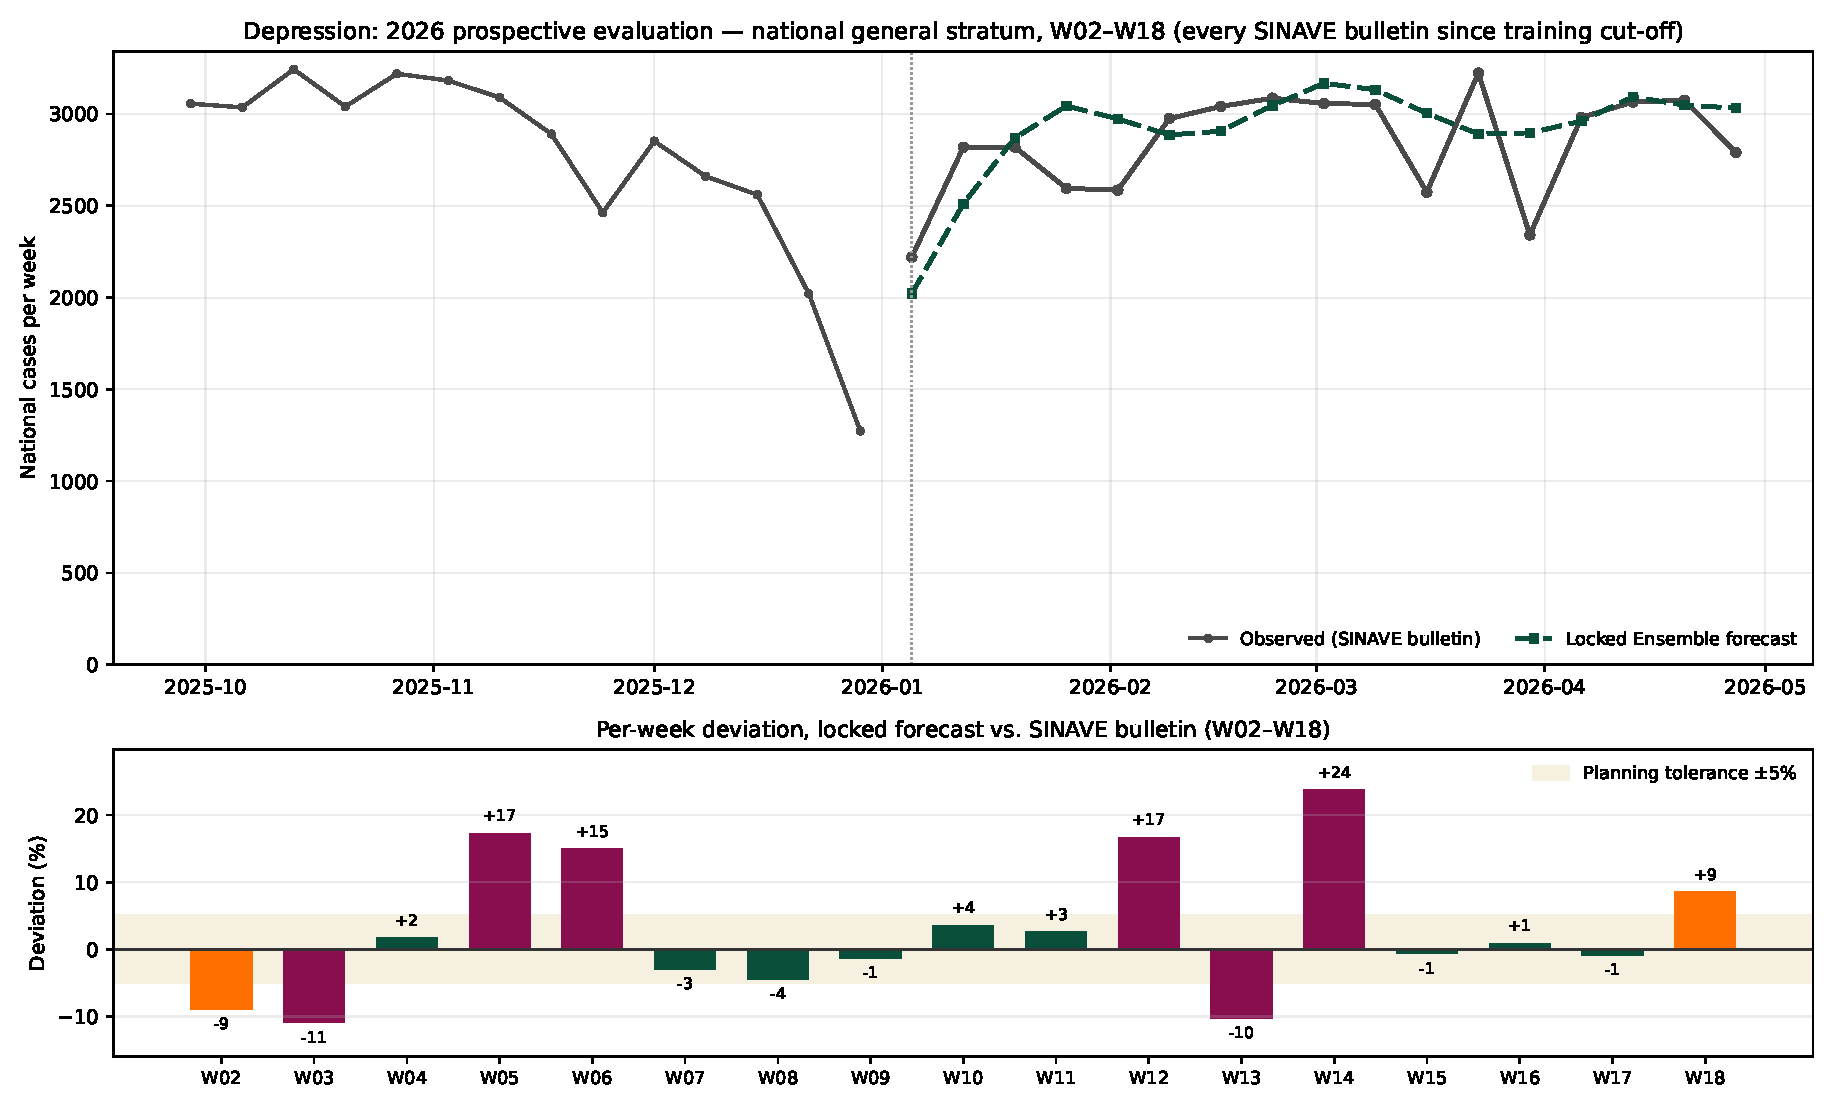
\includegraphics[width=0.86\textwidth]{fig19_validation_2026.pdf}
\caption{2026 out-of-sample evaluation, national general stratum.
(a) Late-2025 context and W01--W18 observed (gray) versus the locked
Ensemble forecast (green); W01 is flagged as incomplete and the W08
planning milestone is annotated. (b) Per-week deviation against the
$\pm5\%$ planning-tolerance band (shaded); bars are colored by
absolute deviation: green within $\pm5\%$, orange between $5\%$ and
$10\%$, and wine above $10\%$.}
\label{fig:validation}
\end{figure}

\paragraph{Aggregate behavior.}
Over the 17 complete weeks W02--W18, the locked forecast attains an
\smape\ of \textbf{6.63\%} (mean \mae\ $=184$ cases per week) and a
cumulative deviation of $+4.40\%$, within the $\pm5\%$ planning
tolerance. The relevant comparator is the CV-period \smape\ for the
same national-general stratum, 8.75\%: the
out-of-sample error is below the in-sample CV error. The weekly errors
have a median absolute percentage error of 3.7\%, below the 6.6\% median of the per-week CV errors, so the forecast generalizes without visible drift. The ranking is robust to the error metric: under a
count-appropriate mean Poisson deviance, the locked Ensemble forecast
is again the best of the four models in this window ($21.7$, against
$31.9$ for Prophet, $32.0$ for DeepAR, and $87.5$ for Stacking).
Consistent with the deployment setting, an empirical 80\% prediction
interval (10th/90th percentiles of post-2021 residuals) covers 15 of 17
validation weeks (88\%; 76\% under a full-history calibration),
bracketing the nominal level rather than reflecting the overconfidence
of a single model's native intervals.

\paragraph{Pairwise comparison.}
A Diebold--Mariano test with the Harvey--Leybourne--Newbold small-sample
correction on the W02--W18 squared-error losses does not reject equal
accuracy between the locked Ensemble and DeepAR ($p=0.15$) or Prophet
($p=0.10$), and indicates that Ensemble is more accurate than Stacking
($p=0.03$); with only seventeen weeks, the test has limited power, so
a non-rejection means insufficient evidence to separate the leading
models, not equivalence.

\paragraph{Largest single-week deviation.}
W14 has the largest single-week deviation ($+26.5\%$), well beyond the
upper quartile of the cross-validation error band.
The value remained at 2{,}341 cases through the manuscript cutoff and
is therefore not a reporting-lag artifact; the four subsequent weeks,
W15--W18, return to an \smape\ of 2.9\%, so the miss does not propagate
into the trajectory. We treat W14 as one observation in the tail of
the in-sample error distribution rather than as evidence of model
drift, and note that the most recent one or two weeks of any bulletin
should still be read with caution because of the documented SINAVE
reporting lag. Week W08, the onset of the February--May saturation
window, deviates by only $+0.2\%$, though the 17-week aggregate is the
more informative summary.

\paragraph{Per-series behavior.}
Cross-validation accuracy does not persist per series out of sample
(Sect.~\ref{sec:results}); Fig.~\ref{fig:oos2026} resolves this by
model and demographic stratum. The cross-validated dominance of the
recurrent model (dashed line) does not survive: out of sample no model
is uniformly best, and the error grows toward the sparse male stratum,
where low weekly counts also inflate \smape\ because of small
denominators---on the scale-free \mase, the same male series remain
near 0.45--0.50 for all four models, well below 1, about twice as
accurate as 52-week seasonal persistence.
This is the regime in which an \emph{auditable, revisable} rule earns
its keep, and Sect.~\ref{ssec:ablation} tests that claim directly
against the frozen deployment.

% ALT-TEXT (accessibility / proofing): Grouped boxplots of out-of-sample 2026 symmetric error (sMAPE, vertical axis) for the four models across three demographic strata (general, women, men). Errors rise from the general to the male stratum and the four models overlap within each stratum, all far above the dashed DeepAR cross-validation median near 6 percent.
\begin{figure}[t]
\centering
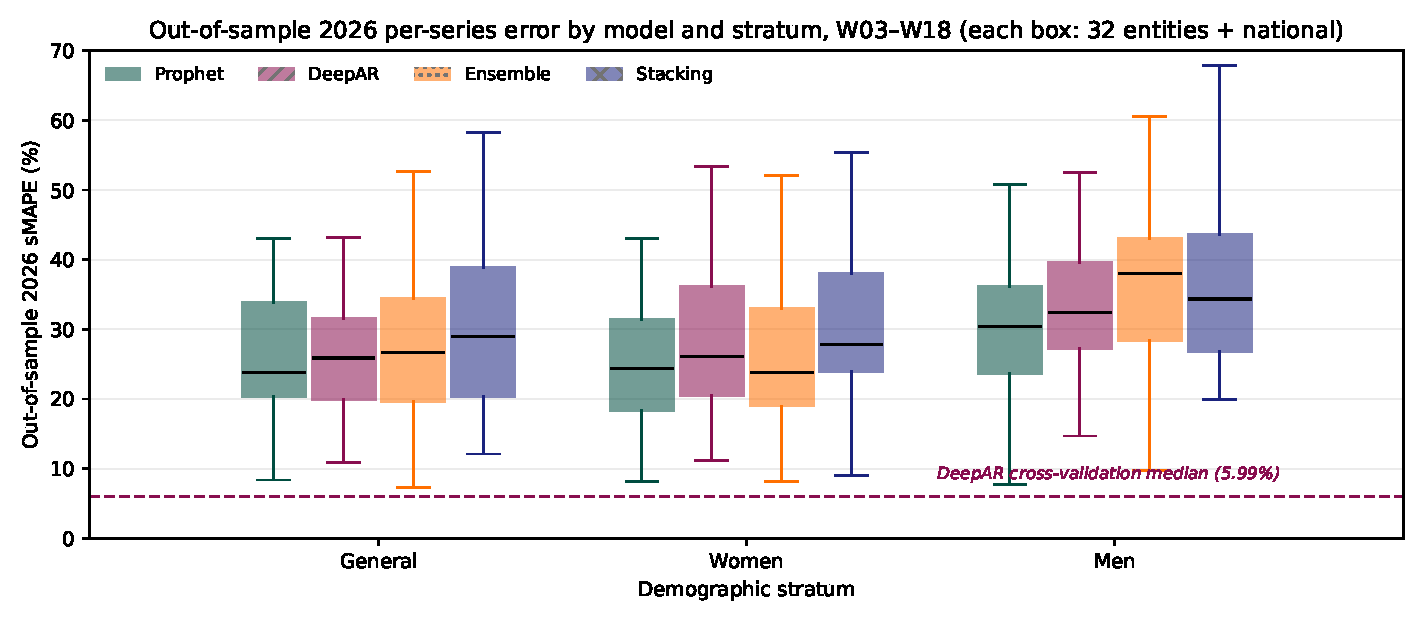
\includegraphics[width=0.95\textwidth]{fig20_oos_perstate.pdf}
\caption{Out-of-sample 2026 per-series symmetric error by model and
demographic stratum; each box pools the 32 federal-entity series with
the national series for that stratum, over the 2026 weeks available at
the production cutoff. On the national-general series alone, Prophet
and the locked Ensemble tie at $13\%$ (national row of the released
per-state table). In cross-validation the recurrent model is
selected for most series at a $5.99\%$ median (dashed line); out of
sample that advantage disappears and the four models converge near
45--48\%, worst on the sparse male stratum. The auditable rule treats
these scores as a revisable signal and reassigns 73 of the 111 series.}
\label{fig:oos2026}
\end{figure}

\subsection{Ablation of the Candidate Pool}
\label{ssec:ablation}

A four-model pool invites a direct question: how much of the result
depends on having four? We re-run the selection rule restricted to each
subset of the pool and rescore the resulting assignments without
refitting---the rule adjudicates among forecasts that were already
locked. Two regimes are separated: \emph{static}, selecting once from
cross-validated evidence as deployed, and \emph{dynamic}, reselecting on
W02--W11 and scoring on the later, unused weeks W12--W18. Selection runs
over all 111 series; scoring runs over the 99 with a direct bulletin
observation, the 12 derived regional series being a sensitivity. Policies
are compared pairwise over the same series (Wilcoxon signed-rank), since
comparing each policy's own reassigned subset would compare different
sets.

\begin{table}[t]
\centering
\caption{Ablation of the candidate pool: median out-of-sample \smape\ (\%)
over the 99 directly observed series, W02--W18. \emph{Static} selects once
from cross-validated evidence; \emph{dynamic} reselects on W02--W11 and is
scored on the unused weeks. $p$: two-sided Wilcoxon signed-rank against
the full pool over the same series. The frozen deployment is the
assignment locked before 2026, and the baseline the dynamic regime must
beat.}
\label{tab:ablation}
\setlength{\tabcolsep}{6pt}
\renewcommand{\arraystretch}{1.1}
\footnotesize
\begin{tabular}{@{}l rr rr@{}}
\toprule
& \multicolumn{2}{c}{\textbf{Static}} & \multicolumn{2}{c}{\textbf{Dynamic}}\\
\cmidrule(lr){2-3}\cmidrule(lr){4-5}
\textbf{Candidate pool} & \smape & $p$ & \smape & $p$\\
\midrule
Full pool (four models)      & 27.9 & ---   & 28.8 & ---\\
\quad without Prophet        & 27.9 & 0.84  & 29.2 & 0.07\\
\quad without DeepAR         & 28.0 & 0.48  & 26.9 & 0.03\\
\quad without Ensemble       & 27.9 & 0.69  & 28.8 & 0.08\\
\quad without Stacking       & 27.9 & 1.00  & 28.9 & 0.31\\
\addlinespace
Prophet alone                & 26.4 & 0.07  & 27.5 & 0.89\\
\midrule
Frozen deployment (baseline) & \multicolumn{2}{c}{---} & 32.6 & ---\\
\bottomrule
\end{tabular}
\end{table}

\paragraph{The pool is not what carries the result.}
Removing any single candidate leaves the static median unmoved: the four
leave-one-out variants fall within $0.1$ points of the full pool and
none approaches significance (Table~\ref{tab:ablation}). This holds even
when the removal reorganizes the assignment completely---dropping DeepAR
moves 107 of 111 selections onto other models and still changes the
median by $0.05$ points. Against a single-model policy the comparison is
no more favorable: Prophet alone attains the best static point estimate,
and we find no evidence that the full selection beats it ($p{=}0.07$;
$p{=}0.06$ on the 111-series sensitivity). We therefore do not claim that
the candidate pool improves accuracy on this panel.

\paragraph{The cross-validated ranking does not transport.}
The direction of the discrepancy matters more than its size. Prophet is
the \emph{worst}-ranked candidate in cross-validation
(Table~\ref{tab:aggmetrics}) and the best in the prospective window. The
evidence the rule selects on is thus not merely noisy out of sample; on
this panel it does not carry the ordering it was selected for. This is
the same phenomenon quantified in Sect.~\ref{sec:results}, isolated to
the selection mechanism itself.

\paragraph{What does hold is revision.}
The dynamic column separates the two claims. Against the frozen
deployment---the assignment actually locked before 2026---reselecting on
prior weeks lowers the median from $32.6\%$ to $28.8\%$ on weeks the
reselection never saw, and every pool tested improves on that baseline.
The gain comes from revising, not from the pool: the full pool does not
beat Prophet alone here either ($p{=}0.89$). The best leave-one-out
variant in this regime, the pool without DeepAR ($26.9\%$, $p{=}0.03$),
is a comparison selected after seeing the outcome, and we do not propose
it as a superior configuration. The framework's value on this panel is
therefore not that four models beat one; it is that a mechanism with an
auditable record detects when a frozen assignment has stopped
transporting and revises it using only observations preceding the
evaluated weeks. A negative ablation is what an auditable design is
supposed to surface, and it bounds how far a cross-validated selection
should be trusted once the signal moves.

% =====================================================================
% =====================================================================
\section{Discussion}
\label{sec:discussion}
% =====================================================================

Combining forecasters with complementary inductive biases and
selecting one model per series through a transparent, revisable rule
provides a principled way to forecast a heterogeneous panel: it
preserves the simpler model when an aggregate series favors it and
reselects models as live data accumulate. The auditable log makes
each locked forecast defensible by a metric rather than by an
architectural preference; we stress that the cross-validation ranking
favoring the recurrent model is a selection signal, not an
out-of-sample guarantee, since per-series accuracy degrades on live
2026 data (Sect.~\ref{sec:results}).

\paragraph{Public-health relevance.}
The 74\%/26\% reported female--male split, broadly echoed by the 2026
forecast (about 73\%/27\%), has planning implications: a service grid
sized to the national mean may underserve
women in absolute terms, while male depression remains plausibly
under-identified. A sex-disaggregated 52-week forecast could support
both proactive capacity allocation for the February--May saturation
window and male-targeted help-seeking campaigns in quieter months. We
emphasize that the data represent \emph{reported incidence}, not
prevalence; the female--male gap is a hypothesis requiring dedicated
epidemiological validation before being used as policy input. This
paper evaluates the framework; it does not describe a deployed
operational system.

\paragraph{Hierarchical reconciliation.}
The three demographic strata are forecast independently, leaving the
${\sim}2.3\%$ general-versus-(women$+$men) incoherence noted in
Sect.~\ref{ssec:demoforecasts}. Applying a minimum-trace
reconciliation~\cite{wickramasuriya2019} to the locked national
forecasts, weighted by the per-stratum cross-validation error
variances, removes the incoherence by construction; the reconciled
national-general series (Table~\ref{tab:validation}, `Recon.'\ column)
shifts the operational forecast by only $1.9\%$ on average and, because
it is already well calibrated, slightly raises the cumulative deviation
($+6.0\%$ vs.\ $+4.40\%$). The independence approximation is thus a
small source of error, and we report the unreconciled forecasts for
transparency.

\paragraph{Limitations.}
Five limitations constrain the conclusions. (i)~Only one condition
(depression) is evaluated; transfer to conditions with different
temporal behavior remains to be demonstrated. (ii)~The per-series
cross-validation metrics of Table~\ref{tab:aggmetrics} are optimistic
relative to live performance, and Sect.~\ref{ssec:ablation} shows the
ranking does not transport. The out-of-sample claim therefore rests on
the national-aggregate prospective evaluation and on the revision
experiment, not on the cross-validation medians. (iii)~The headline prospective
evaluation is at the national-aggregate stratum over an early-2026
window (W01--W18); a per-state out-of-sample table over the same window
is released with the source code, but a per-state \emph{full-year}
evaluation is still pending. (iv)~The
most recent bulletins are subject to reporting-lag revision, so the
latest one or two weeks are provisional. (v)~The framework has not
been externally validated outside SINAVE/Mexico. (vi)~SINAVE is a
passive, facility-based system, so the panel measures \emph{reported}
incidence: it counts episodes that reached care and were coded, not
episodes that occurred. Two consequences bear on generalizability.
Diagnostic and reporting capacity differs across federal entities, so
part of the level difference between states reflects surveillance
capacity rather than epidemiology; and care-seeking differs by sex, which
is the most likely source of the male shortfall noted in
Sect.~\ref{ssec:data}. A model fitted to these series therefore learns
the reporting process together with the disease process, and the
selection rule inherits both. This does not invalidate the forecasts for
planning---services are sized against reported demand, which is what the
panel measures---but it does mean the framework should not be read as
forecasting community-level incidence, and that transfer to a system with
different case-ascertainment rules must be demonstrated, not assumed.

\paragraph{Future work.}
We plan to extend the framework to additional CIE-10 codes in the
SINAVE catalog, to report a full-year per-state prospective evaluation,
to add tuned SARIMA and N-BEATS/N-HiTS baselines, and to
pursue external validation. A further direction is to make the
\emph{forecasts} explainable, not only the selection. The rule explains
which model was chosen and on what evidence, but not why that model
expects a given trajectory; post-hoc attribution over the tree-based
hybrids and saliency over the recurrent model's context window would let
a planner see which lags and calendar effects drive a specific weekly
figure. That is a different guarantee from the one offered here, and we
treat it as complementary rather than as a refinement of the rule.

% =====================================================================
\section{Conclusions}
\label{sec:conclusions}
% =====================================================================

We presented an empirical study of multi-model, per-series forecast
selection for weekly depression incidence at federal-entity
granularity in Mexico, comparing a structural model, a global
probabilistic recurrent network, and two tree-based hybrids under a
deterministic, auditable, and revisable selection rule. Cross-validation on more than a decade of SINAVE data, across a
nationwide panel of series and demographic strata, selects the
recurrent model (DeepAR) for the large majority of federal-entity
series, while the rule retains simpler models where aggregation
favors them. We
explicitly treat this ranking as an in-sample selection signal: on
live 2026 data the per-series advantage narrows and the framework
reselects, so our out-of-sample evidence is the prospective national
evaluation, not the cross-validation figures. We are not aware of prior
work that applies a multi-model framework with auditable, revisable
per-series model selection to psychiatric surveillance at
federal-entity granularity in a Latin American country. The framework
is a research prototype; future work will broaden the set of conditions,
baselines, and prospective horizons evaluated.

% =====================================================================
\section*{Ethics and Data Availability}
% =====================================================================
The SINAVE bulletin reports aggregate weekly case counts at the
federal-entity level, stratified by sex. All analyses were performed
on these aggregate cells, and no cell corresponds to an individual
patient; therefore, no informed consent or review-board approval was
required.
The data are published as open data by the Direcci\'on General de
Epidemiolog\'ia, Secretar\'ia de Salud, and were retrieved from the
public SINAVE portal on 2026-04-15~\cite{sinave2026}; redistribution
is governed by the bulletin's open-data terms.

% >>> CAMERA-READY credits block (active). Remove for REVIEW version.
\begin{credits}
\subsubsection{\ackname}
The authors thank Drs.~Lina D\'iaz-Castro (Instituto Nacional de
Psiquiatr\'ia Ram\'on de la Fuente Mu\~niz) and Silvia Magali
Cuadra-Hern\'andez (Instituto Nacional de Salud P\'ublica) for
epidemiological interpretation. The Tecnol\'ogico de Monterrey
M.Sc.\ in Applied Artificial Intelligence (MNA) program provided
institutional support.

\subsubsection{\discintname}
The authors declare no competing interests. This work was developed
independently under the MNA program, with no external funding and no
proprietary data or computing resources.
\end{credits}

% =====================================================================
\appendix
\section{Implementation and Reproducibility Details}
\label{app:impl}
% =====================================================================
The four models share a single interface and are configured from
hierarchical YAML files under OmegaConf. The framework runs on
Python~3.12 with GluonTS~0.15 (PyTorch~2.5), Prophet~1.1,
XGBoost~2.0, LightGBM~4.3, scikit-learn~1.4, and pandas~2.2; DeepAR
trains on one NVIDIA~T4 GPU and the remaining models on CPU. Run-to-run reproducibility is enforced by
fixing every seed source---\texttt{torch}, \texttt{numpy},
\texttt{random}, and the tree libraries' sampling seeds---at~42 and
enabling deterministic cuDNN kernels. Table~\ref{tab:hparams} lists the
per-model hyperparameters; the configuration files, the model-selection
pseudocode, and the per-state out-of-sample table are released with the
source code.

\begin{table}[t]
\centering
\caption{Principal hyperparameters per model, fixed before the 2026
evaluation window.}
\label{tab:hparams}
\setlength{\tabcolsep}{5pt}
\renewcommand{\arraystretch}{1.12}
\footnotesize
\begin{tabular}{@{}l@{\hspace{8pt}}p{0.78\textwidth}@{}}
\toprule
\textbf{Model} & \textbf{Principal hyperparameters} \\
\midrule
DeepAR & 2 layers $\times$ 80 cells; context 104 wk; horizon 52;
         dropout 0.15; Student-$t$ output; Adam
         $\eta{=}5{\times}10^{-4}$, $\lambda_2{=}10^{-6}$; batch 32;
         $\leq$300 epochs; early stop (patience 15). \\
\addlinespace
Prophet & rate per 100k, $\log(1{+}y)$; changepoint prior
          $\in\{0.01,0.03,0.05\}$; seasonality prior
          $\in\{0.025,0.05,0.1,0.5\}$ (12-point grid under temporal CV). \\
\addlinespace
Ensemble & XGBoost on calendar/lags $\{1,2,4,8,13,26,52\}$/rolling
           stats; blend weight learned on out-of-fold predictions. \\
\addlinespace
Stacking & Prophet $+$ ETS $+$ LightGBM experts; nonnegative
           ElasticNet ($\alpha{=}1.0$, \texttt{l1\_ratio}${=}0.5$). \\
\bottomrule
\end{tabular}
\end{table}

% =====================================================================
% References (Springer MathPhSci / splncs04 style, alphabetical order)
% =====================================================================
\begin{thebibliography}{99}

\bibitem{albert2015}
Albert, P.R.: Why is depression more prevalent in women?
J.\ Psychiatry Neurosci.\ \textbf{40}(4), 219--221 (2015).
\url{https://doi.org/10.1503/jpn.150205}

\bibitem{alexandrov2020}
Alexandrov, A., Benidis, K., Bohlke-Schneider, M., Flunkert, V.,
Gasthaus, J., Januschowski, T., et al.: GluonTS: probabilistic and
neural time series modeling in Python. J.\ Mach.\ Learn.\ Res.\
\textbf{21}(116), 1--6 (2020).
\url{http://jmlr.org/papers/v21/19-820.html}

\bibitem{ansari2024chronos}
Ansari, A.F., Stella, L., T\"urkmen, C., Zhang, X., Mercado, P., Shen,
H., et al.: Chronos: learning the language of time series. Trans.\ Mach.\
Learn.\ Res.\ (2024). \url{https://doi.org/10.48550/arXiv.2403.07815}

\bibitem{benidis2022}
Benidis, K., Rangapuram, S.S., Flunkert, V., Wang, Y., Maddix, D.,
T\"urkmen, C., et al.: Deep learning for time series forecasting:
tutorial and literature survey. ACM Comput.\ Surv.\ \textbf{55}(6),
1--36 (2022). \url{https://doi.org/10.1145/3533382}

\bibitem{box2015}
Box, G.E.P., Jenkins, G.M., Reinsel, G.C., Ljung, G.M.: Time Series
Analysis: Forecasting and Control, 5th edn. John Wiley \& Sons,
Hoboken (2015)

\bibitem{challu2023nhits}
Challu, C., Olivares, K.G., Oreshkin, B.N., Garza Ramirez, F.,
Mergenthaler Canseco, M., Dubrawski, A.: N-HiTS: neural hierarchical
interpolation for time series forecasting. In: Proceedings of the AAAI
Conference on Artificial Intelligence, vol.~37, no.~6, pp.~6989--6997
(2023). \url{https://doi.org/10.1609/aaai.v37i6.25854}

\bibitem{chen2016}
Chen, T., Guestrin, C.: XGBoost: a scalable tree boosting system. In:
Proceedings of the 22nd ACM SIGKDD International Conference on
Knowledge Discovery and Data Mining (KDD), pp.~785--794. ACM,
San Francisco (2016). \url{https://doi.org/10.1145/2939672.2939785}

\bibitem{chimmula2020}
Chimmula, V.K.R., Zhang, L.: Time series forecasting of COVID-19
transmission in Canada using LSTM networks. Chaos Solitons Fractals
\textbf{135}, 109864 (2020).
\url{https://doi.org/10.1016/j.chaos.2020.109864}

\bibitem{cramer2022}
Cramer, E.Y., Ray, E.L., Lopez, V.K., Bracher, J., Brennen, A.,
Castro Rivadeneira, A.J., et al.: Evaluation of individual and ensemble
probabilistic forecasts of
COVID-19 mortality in the United States. Proc.\ Natl.\ Acad.\ Sci.\
USA \textbf{119}(15), e2113561119 (2022).
\url{https://doi.org/10.1073/pnas.2113561119}

\bibitem{dash2024}
Dash, S., Giri, S.K., Mallik, S., Pani, S.K., Shah, M.A., Qin, H.:
Predictive healthcare modeling for early pandemic assessment leveraging
deep auto regressor neural prophet. Sci.\ Rep.\ \textbf{14}, 5287
(2024). \url{https://doi.org/10.1038/s41598-024-55973-y}

\bibitem{sinave2026}
Direcci\'on General de Epidemiolog\'ia (DGE), Secretar\'ia de Salud,
M\'exico: SINAVE Bolet\'in Epidemiol\'ogico.
\url{https://www.gob.mx/salud/acciones-y-programas/direccion-general-de-epidemiologia-boletin-epidemiologico}
(accessed 2026-04-15)

\bibitem{garciapacheco2024}
Garc\'ia-Pacheco, J.\'A., Torres-Ortega, M.L., Borges, G.: The burden
of mental disorders in Mexico, 1990--2019: mental and neurological
disorders, substance use, suicides, and related somatic disorders.
Span.\ J.\ Psychiatry Ment.\ Health \textbf{17}(2), 64--70 (2024).
\url{https://doi.org/10.1016/j.rpsm.2021.06.005}

\bibitem{godahewa2023}
Godahewa, R., Bergmeir, C., Webb, G.I., Montero-Manso, P.: An accurate
and fully-automated ensemble model for weekly time series forecasting.
Int.\ J.\ Forecast.\ \textbf{39}(2), 641--658 (2023).
\url{https://doi.org/10.1016/j.ijforecast.2022.01.008}

\bibitem{hewamalage2021}
Hewamalage, H., Bergmeir, C., Bandara, K.: Recurrent neural networks
for time series forecasting: current status and future directions.
Int.\ J.\ Forecast.\ \textbf{37}(1), 388--427 (2021).
\url{https://doi.org/10.1016/j.ijforecast.2020.06.008}

\bibitem{hyndman2018forecasting}
Hyndman, R.J., Athanasopoulos, G.: Forecasting: Principles and
Practice, 2nd edn. OTexts, Melbourne (2018).
\url{https://otexts.com/fpp2/}

\bibitem{hyndman2006}
Hyndman, R.J., Koehler, A.B.: Another look at measures of forecast
accuracy. Int.\ J.\ Forecast.\ \textbf{22}(4), 679--688 (2006).
\url{https://doi.org/10.1016/j.ijforecast.2006.03.001}

\bibitem{hyndman2008}
Hyndman, R.J., Koehler, A.B., Ord, J.K., Snyder, R.D.: Forecasting
with Exponential Smoothing: The State Space Approach. Springer, Berlin
(2008). \url{https://doi.org/10.1007/978-3-540-71918-2}

\bibitem{ke2017}
Ke, G., Meng, Q., Finley, T., Wang, T., Chen, W., Ma, W., et al.:
LightGBM: a highly efficient gradient boosting decision tree. In:
Advances in Neural Information Processing Systems (NeurIPS), vol.~30,
pp.~3146--3154 (2017).
\url{https://proceedings.neurips.cc/paper/2017/hash/6449f44a102fde848669bdd9eb6b76fa-Abstract.html}

\bibitem{lim2021}
Lim, B., Zohren, S.: Time-series forecasting with deep learning: a
survey. Philos.\ Trans.\ R.\ Soc.\ A \textbf{379}(2194), 20200209
(2021). \url{https://doi.org/10.1098/rsta.2020.0209}

\bibitem{makridakis2020}
Makridakis, S., Spiliotis, E., Assimakopoulos, V.: The M4 Competition:
100{,}000 time series and 61 forecasting methods. Int.\ J.\ Forecast.\
\textbf{36}(1), 54--74 (2020).
\url{https://doi.org/10.1016/j.ijforecast.2019.04.014}

\bibitem{makridakis2022}
Makridakis, S., Spiliotis, E., Assimakopoulos, V.: The M5 accuracy
competition: results, findings, and conclusions. Int.\ J.\ Forecast.\
\textbf{38}(4), 1346--1364 (2022).
\url{https://doi.org/10.1016/j.ijforecast.2021.11.013}

\bibitem{nie2023patchtst}
Nie, Y., Nguyen, N.H., Sinthong, P., Kalagnanam, J.: A time series is
worth 64 words: long-term forecasting with transformers. In:
International Conference on Learning Representations (ICLR) (2023).
\url{https://doi.org/10.48550/arXiv.2211.14730}

\bibitem{reich2019}
Reich, N.G., Brooks, L.C., Fox, S.J., Kandula, S., McGowan, C.J., Moore,
E., et al.: A collaborative multiyear, multimodel assessment of seasonal
influenza forecasting in the United States. Proc.\ Natl.\ Acad.\ Sci.\
USA \textbf{116}(8), 3146--3154 (2019).
\url{https://doi.org/10.1073/pnas.1812594116}

\bibitem{salinas2020}
Salinas, D., Flunkert, V., Gasthaus, J., Januschowski, T.: DeepAR:
probabilistic forecasting with autoregressive recurrent networks.
Int.\ J.\ Forecast.\ \textbf{36}(3), 1181--1191 (2020).
\url{https://doi.org/10.1016/j.ijforecast.2019.07.001}

\bibitem{santomauro2021}
Santomauro, D.F., Mantilla Herrera, A.M., Shadid, J., Zheng, P.,
Ashbaugh, C., Pigott, D.M., et al.: Global prevalence and burden of
depressive and
anxiety disorders in 204 countries and territories in 2020 due to the
COVID-19 pandemic. Lancet \textbf{398}(10312), 1700--1712 (2021).
\url{https://doi.org/10.1016/S0140-6736(21)02143-7}

\bibitem{taylor2018}
Taylor, S.J., Letham, B.: Forecasting at scale. Am.\ Stat.\
\textbf{72}(1), 37--45 (2018).
\url{https://doi.org/10.1080/00031305.2017.1380080}

\bibitem{wickramasuriya2019}
Wickramasuriya, S.L., Athanasopoulos, G., Hyndman, R.J.: Optimal
forecast reconciliation for hierarchical and grouped time series
through trace minimization. J.\ Am.\ Stat.\ Assoc.\ \textbf{114}(526),
804--819 (2019).
\url{https://doi.org/10.1080/01621459.2018.1448825}

\bibitem{wolpert1992}
Wolpert, D.H.: Stacked generalization. Neural Netw.\ \textbf{5}(2),
241--259 (1992).
\url{https://doi.org/10.1016/S0893-6080(05)80023-1}

\end{thebibliography}

\end{document}
